\documentclass[final,3p]{CSP}
\usepackage{amssymb}
\usepackage{changepage}
\usepackage{float}
\usepackage{hyperref}
\usepackage{url}
\usepackage{afterpage}
\usepackage{natbib}
\usepackage{setspace}
\usepackage{fancyhdr}
\pagestyle{fancy}
\fancyhf{}

\def\Student{Ashish Sehrawat}
\def\Title{THESIS PROJECT PROPOSAL}
\def\Prog{Doctorado en Ciencias (F\'{i}sica) }
\def\Dept{Departamento de Investigac\'{i}on en Fis\'{i}ca}
\def\Director{Dr. Jos\'{e} Feliciano Ben\'{i}tez Rubio}
\def\ProjectTitle{Study of the Higgs boson production in association with a single top quark in proton collisions at the Large Hadron Collider}
\def\ResearchLine{Astrof\'{i}sica, Cosmolog\'{i}a y F\'{i}sica de Part\'{i}culas}


\newcommand{\SubItem}[1]{
    {\setlength\itemindent{15pt} \item[-] #1}
}


%%header and footer
\lhead{\Student}
\rhead{\Title}
\lfoot{\Dept}
\rfoot{Page \thepage}
\setlength{\headsep}{0.2in}
\renewcommand{\footrulewidth}{0.4pt}% default is 0pt


\begin{document}

%%%%Title Page
\begin{titlepage}
  \centering
  \hspace{0pt}
  \vfill
        {\scshape\Large \Title \par}

	\vspace{2cm}
        \begin{adjustwidth}{2cm}{2cm}{
            TITLE:\par
            {\large \ProjectTitle \par}
          }
        \end{adjustwidth}

	\vspace{0.5cm}
        \begin{adjustwidth}{2cm}{2cm}{
            RESEARCH LINE: \par
            \ResearchLine \par}
        \end{adjustwidth}

        
        \vspace{4cm}
        {\underline{\hspace{8cm}}\par}
	{\scshape\large \Student \par}
        {Student\par}

        \vspace{1cm}
        {\underline{\hspace{8cm}}\par}
	{\Director \par}
        {Director\par}

        \vspace{1cm}
        {\Prog \par}
        {\Dept \par}
        {Universidad de Sonora \par}

        \vspace{4cm}
	{\today}

\hspace{0pt}
\vfill

\end{titlepage}


%%%%% white page for print out
\shipout\null


%%%% Abstract Page
\newpage
\hspace{2pt}
\vfill

\begin{adjustwidth}{1cm}{1cm}

  \begin{center}
    {\Large \ProjectTitle \par}
    \vspace{1cm}
    {\itshape\textbf{Abstract}\par}
  \end{center}
  
  \vspace{1 cm}
 
  
\onehalfspacing This research project proposes to study the unobserved production channel of the Higgs boson in associated with a single top quark (tH) using Higgs boson decay to multilepton final state. The dataset collected during the Run II (2015-2018) of Large Hadron Collider (LHC) will be used corresponding to an integrated luminosity of 150 $fb^{-1}$. Increasing the collider luminosity is expected to increase the number of event for this Higgs boson production mode. The measurement of this production mode has ramifications for other measurements related to coupling parameter $y_t$ of the top quark and the Higgs boson which is part of the physics program of the international CMS and ATLAS collaborations. Previous measurements using dataset with an integrated luminosity 36 $fb^{-1}$ has put an upper limit of 2.04 pb on the production cross section which is far from standard model predicted value of 0.077 pb. We plan to obtain more stringent upper limits on the production cross section and get constraints on the Higgs top quark coupling parameter $y_t$. \par

\end{adjustwidth}

\hspace{2pt}
\vfill

%%%%%% Begin the body
\newpage
\section{BACKGROUND}


\onehalfspacing The standard model (SM) of particle physics is so far the best theoretical model to describe the interaction of elementary 
particles using three of the four fundamental forces of nature which are electromagnetic force, strong nuclear force and the 
weak nuclear force. Gravitational force is neglected as the strength of this force is very weak at the scales over which 
elementary particle interact with each other. The standard model (SM) of particle physics is divided into two categories, 
bosonic sector and fermionic sector. Bosonic sector contain particles called bosons which mediate the fundamental forces of 
nature and the fermionic sector contain particles called fermions which make up all the matter in our universe. SM has three 
generations of matter (fermions) particles. The first generation of fermions consists of up (u) quark, down (d) quark, electron 
and electron neutrino, second generation consist of charm (c) quark, strange (s) quark, muon and muon neutrino and the third 
generation of matter particles has top (t) quark, bottom (b) quark, tau and tau neutrino. The bosonic sector consist of gauge 
bosons like gluon, photon, $W^{\pm}$, $Z^0$ which mediate strong nuclear force, electromagnetic force and weak nuclear force respectively. There is one more particle in the standard model called the Higgs Boson which gives mass to SM particles via electroweak symmetry breaking mechanism \cite{Chatrchyan:2012xdj}. All the standard model particles are shown in Figure 1. Higgs boson can be produced at the particle colliders like the Large Hadron Collider (LHC) in Geneva, Switzerland.

\begin{figure}[H]
	\centering
	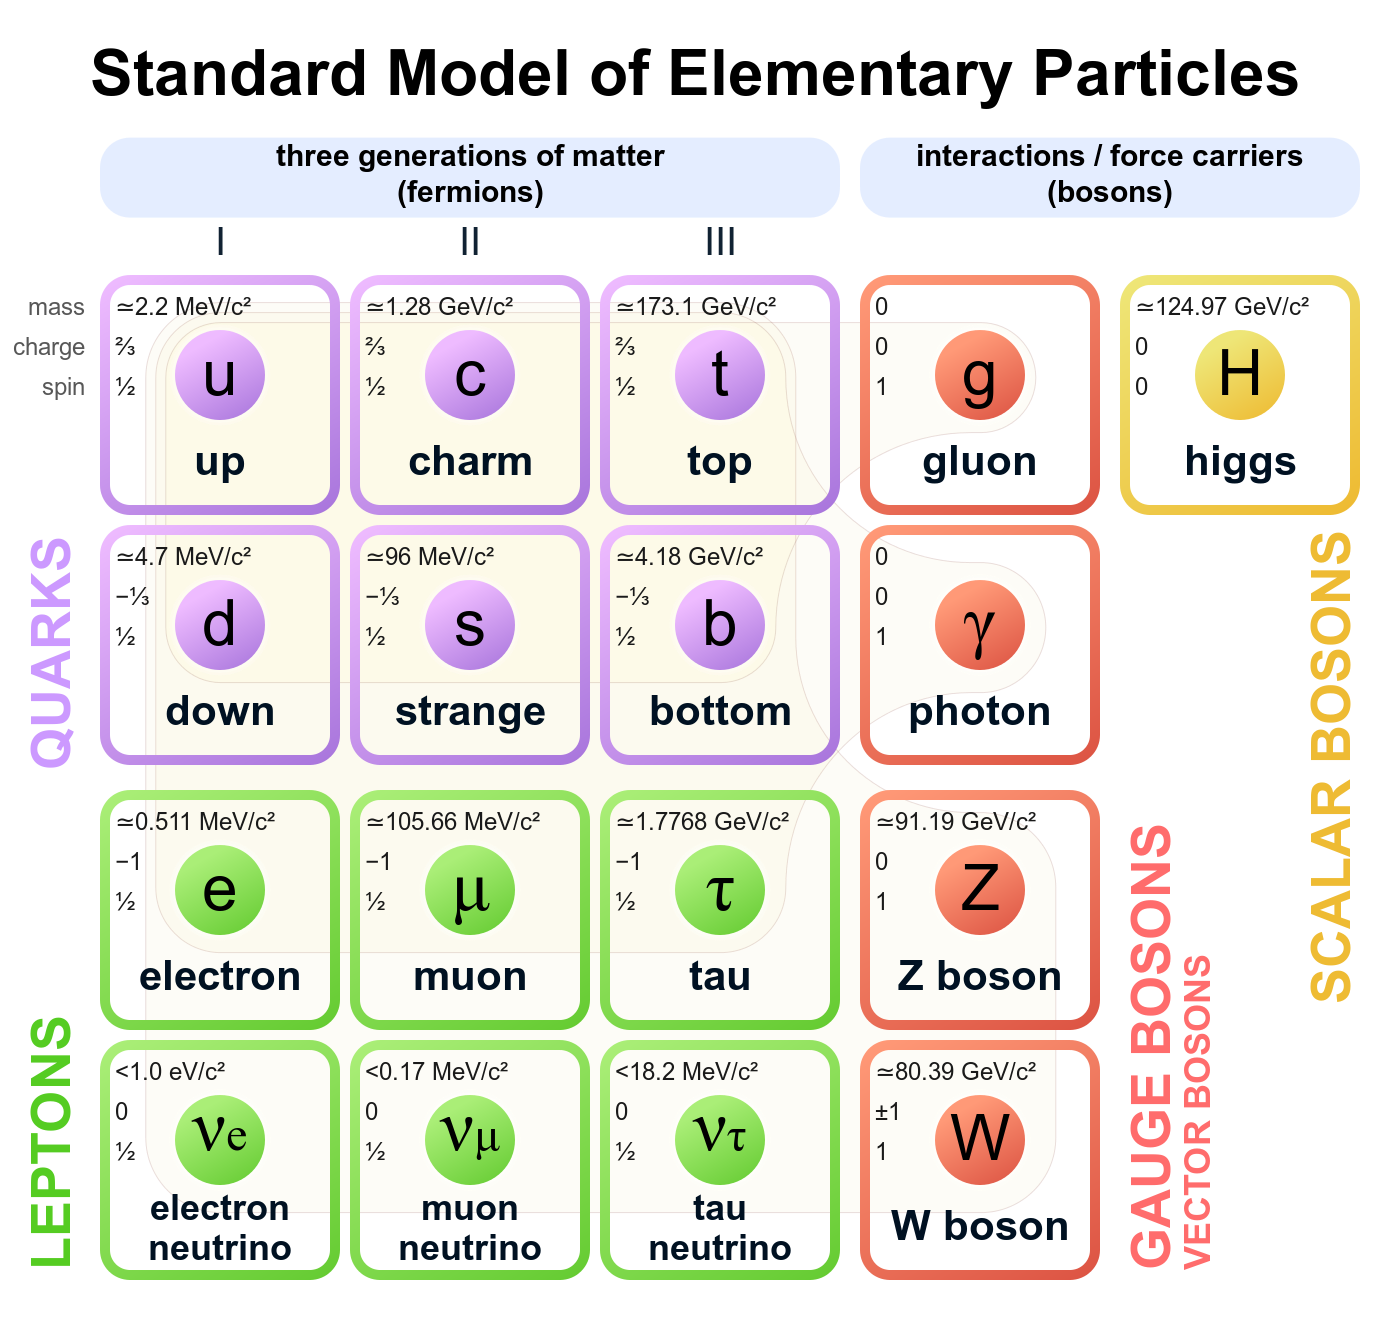
\includegraphics[width= 0.5 \columnwidth]{./sm.png}
	\caption{Elementary particles in standard model of particle physics with their mass, spin and charge.}
	\label{figure 1}
\end{figure}

% \newpage

There are various production modes of Higgs boson like the gluon gluon fusion (ggF), vector boson fusion (VBF), Higgs 
production in association with vector boson (VH, V = $W^{\pm}$ or Z), Higgs production with top quark and top anti-quark ($t\bar{t}H$) and Higgs 
production in association with a single top quark and a quark jet (tHq). Each production channel has its own importance to probe the 
various properties like spin, parity and the coupling strength parameters of Higgs boson to fermions and bosons. The main production mode of Higgs boson at LHC is 
gluon gluon fusion (ggF). As bosons like gluons and photons are massless, they do not interact directly with the Higgs boson 
and processes like ggF or Higgs boson decay to pair of photons are not possible at tree level and can only proceed via loop 
diagrams which involve $W^{\pm}$ boson, top quark or bottom quark in the loop. The Higgs boson can also decay to other particles and these decay 
channels have different branching ratios which are computed using the partial decay widths. Higgs boson can decay to a pair of $W^{\pm}$ bosons, Z bosons, photons, bottom quarks, 
muons and electrons. Higgs boson can also decay to Z boson and a photon. The important SM Higgs Boson production modes are shown in Figure 2. The production cross section and branching ratios of various decay channels of Higgs boson are shown in Figure 3.

%\afterpage{
\begin{figure}[H]
	\centering
	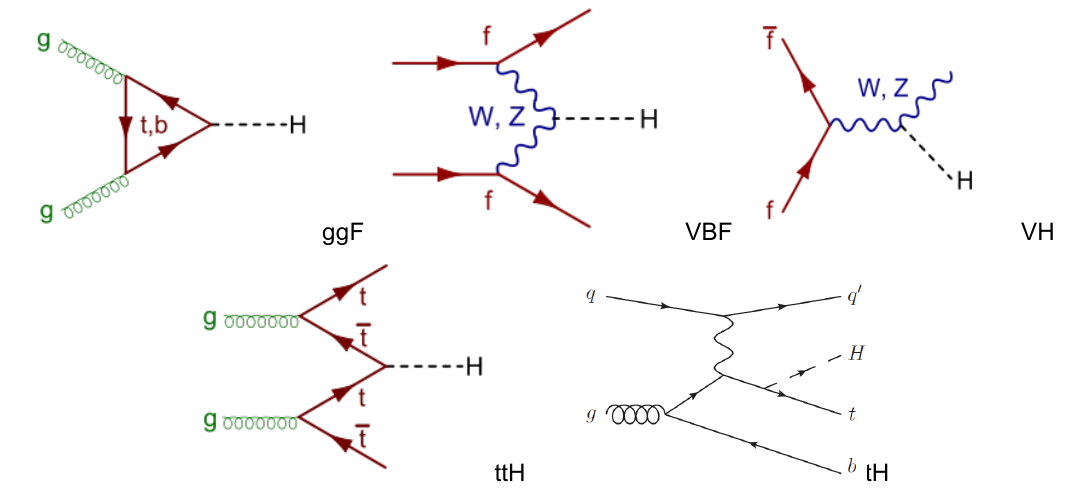
\includegraphics[width=\columnwidth]{./pg.png}
	\caption{Important production processes of Standard model Higgs boson ggF, VBF, VH, ttH and tH in proton collisions.}
	\label{figure 2}
\end{figure}


\begin{figure}[H]
  \centering
   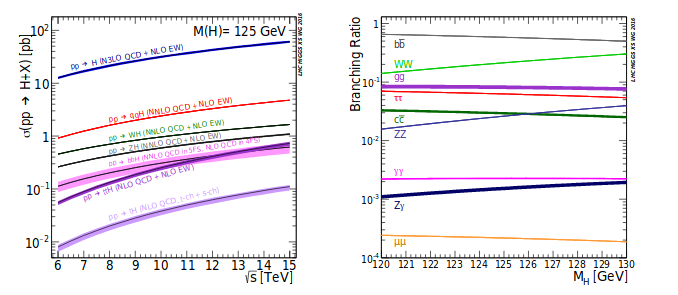
\includegraphics[scale=0.7]{./cd2.png}
  \caption{Standard model Higgs boson production cross section with center of mass energy and branching ratios for various decay channels \cite{Tanabashi:2018oca}.}
   \label{figure 3}
\end{figure}
\clearpage

 \newpage

The Standard Model (SM) of particle physics has successfully described most of the experimental data till now but a very large 
number of free-parameters and the fine tuning related to these parameters suggest new physics beyond SM as mentioned below.
\begin{itemize}
\item{Fine structure constant $\alpha$},
\item{Weinberg angle or the weak mixing angle $\theta_W$},
\item{The coupling constant of strong interaction $\alpha_s$},
\item{Electroweak symmetry breaking energy scale v},
\item{ Higgs potential self coupling $\lambda$ or the Higgs mass $m_H$},
\item{Three weak mixing angles and the CP-violating phase $\delta$ of the CKM matrix which tells us how quarks of different flavor mix with each other},
\item{Nine yukawa couplings $y_i$ (i = 1 to 9) which determine the mass of nine charged fermions}.
\end{itemize}
 The fine 
tunings related to the Higgs 
mass and the free parameters in SM suggests new physics beyond Standard model (BSM). There are lot of specific 
BSM theories and most of these 
models involve new heavy particles. In order to identify which new physics lies beyond the 
electroweak (EW) scale, the new parameters 
of such theories may be constrained by the actual low energy experiments.

There is another approach immitating 
Fermi's treatment of beta decay 
which consists of considering the SM as the first order approximation of the actual theory 
and by completing it with a series 
of higher dimensional operators. When the electroweak symmetry breaking takes place well 
below the mass of the new particles, 
the BSM physics is taken into account at the EW scale and below by adding higher dimensional 
operators to the SM Lagrangian. 
They are built out of SM fields and supposed to be invariant under its gauge group which is $SU(3)_C \times SU(2)_L \times U(1)_Y$.
%Those 
%operators are the low-energy residue 
%of the high energy theory. This approach does not pretend to guess the complete high-energy 
%model and it is based solely on 
%the symmetry of the  theory. The operators are general and the only model dependence is 
%encoded in the size of the operator
%coefficients, which is to be set from experiments. The Higgs boson and fermions (quarks and leptons) coupling will deviate from the standard 
%model predictions if these higher 
%dimensional operators are present in low energy effective SM theory. We can consider 
%anomalous Higgs and Higgs-gauge effective 
%dimension 6 operators like $-\frac{1}{3}(\phi^{\dagger}\phi)^3$, $\frac{1}{2} \partial_{\mu} 
%(\phi^{\dagger} \phi) 
%\partial^{\mu}(\phi^{\dagger} \phi)$ and $(\phi^{\dagger} \phi)(D_{\mu} \phi)^{\dagger} 
%(D^{\mu} \phi)$ to calculate the 
%deviation of Higgs boson-fermion couplings from SM. The first operator $-\frac{1}{3}(\phi^{\dagg%er}\phi)^3$ shift the minimum of 
%the Higgs potential. Also as there 
%will be rescaling of the Higgs field due to the introduction of these operators in the 
%potential term, Higgs-fermion (quarks 
%and leptons) couplings will be modified.
The yukawa coupling of top quark with Higgs boson will be modified due to the presence of such higher dimensional operators.

\begin{figure}[ht]
	\centering
	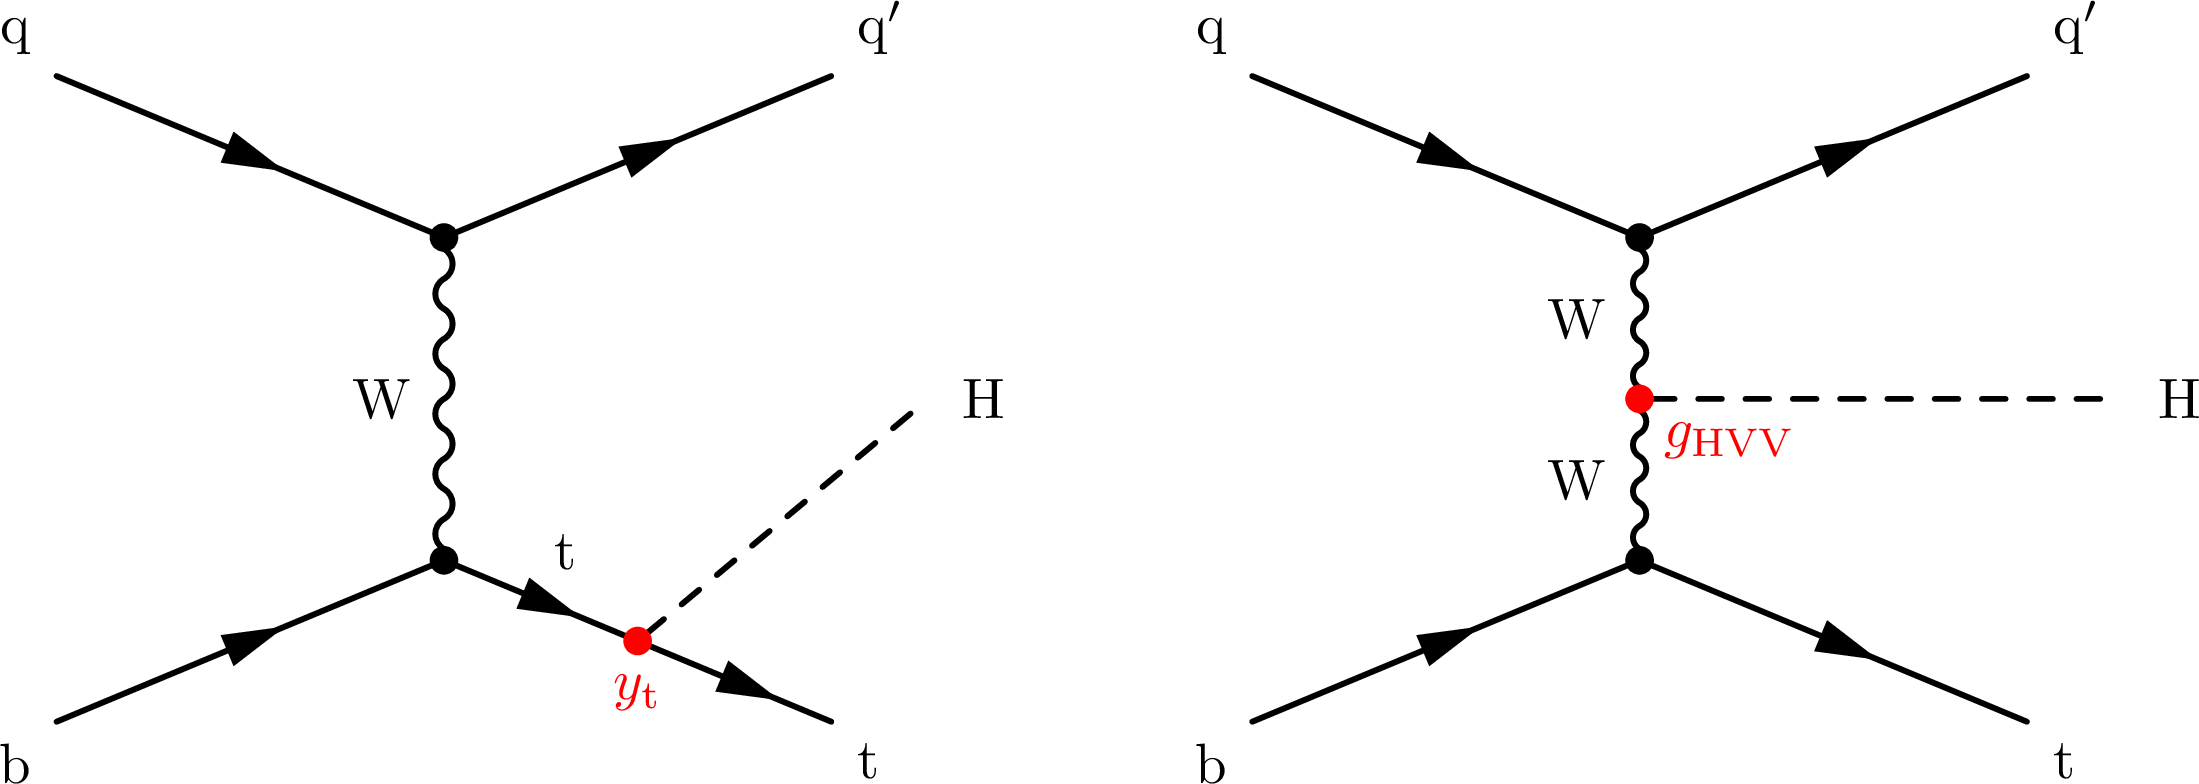
\includegraphics[width=\columnwidth]{./cms.png}
	\caption{Leading order Feynman diagrams for the associated production of a single top quark and a Higgs boson in the t channel, where the Higgs boson couples either to the top quark (left) or the W boson (right).}
	\label{figure 4}
\end{figure}


The production of Higgs boson in association with single top quark is one of the rare Higgs 
boson production mode \cite{sirunyan2019search}. As the top 
quark is the heaviest fundamental particle in the standard model, due to its large mass, the 
top quark decay before 
hardronization which allow the possibility to reconstruct top quark from its decay products 
unlike the lighter quarks which 
undergo hardronization and are seen as bundles of particles in detector called jets. The most 
probable decay of the top quark is 
into bottom (b) quark and $W^{\pm}$ boson \cite{{Tanabashi:2018oca}}. Using b-jet tagging algorithms, the jet originating from 
b-quark can be reconstructed to 
identity the top quark. In SM, the couplings of the Higgs boson to fermions (quarks and leptons) known as Yukawa couplings are proportional to the mass 
of the fermions. Thus heavy quarks like top, bottom and charm couple strongly to Higgs boson 
which means that out of all known 
quarks, top quark couple most strongly to the Higgs boson. So, it has a large value of Yukawa 
coupling $y_t$ \cite{Aad_2016}. That is why the 
Yukawa coupling of the top quark with the Higgs boson $y_t$ has lot of importance as any 
deviation from standard model prediction might give an indication of new physics. The two 
processes at LHC which will allow us to directly probe the Yukawa 
coupling between Higgs boson and top quark are Higgs boson production in association with top 
quark pair ($t\bar{t}H$) via 
strong interaction and the production of single top quark with a Higgs boson (tH). As tH 
occur via electroweak interaction, it 
is more rare than t$\bar{t}$H production \cite{Sirunyan:2018ygk}. The Higgs boson in the tH channel can be radiated 
off by a $W^{\pm}$ boson or by a top quark as shown in Figure 4.

 These two processes in standard model have destructive interference which allow us to 
probe the relative sign between 
the coupling of top quark with Higgs boson $y_t$ and the coupling of $W^{\pm}$ boson to the Higgs 
boson $g_{HWW}$ \cite{Sirunyan:2018lzm}. If the Yukawa coupling between top quark and Higgs boson $y_t$ deviate from the SM 
prediction or even if $y_t$ has a negative sign, both would cause a strong increase in the tH 
production cross section which is a special property of tH production channel making it an 
interesting production channel to probe using LHC 2016, 2017 and 2018 data \cite{farina2013lifting}. The coupling 
strength modifier $\kappa_t$ is defined as $\kappa_t = \frac{y_t}{y^{SM}_t}$ which will tell 
us the deviation of $y_t$ from the SM prediction. 

The LHC is sensitive to an anomalous Higgs coupling to the top quark in the Higgs boson-top quark associated production mode. 
The anomalous coupling will arise when we add interaction terms (dimension 6 operators in effective SM theory) in the Higgs potential.
As there is strong destructive inteference in the t-channel for the standard model  couplings, this production mode is sensitive to both the sign and the magnitude of any coupling beyond the SM between Higgs  boson and top quark induced by higher dimensional operators in effective beyond SM theory \cite{sirunyan2019search}.

Until the 90's the existence of almost all the particles of the SM were confirmed except the top quark and the Higgs boson. 
These had eluded previous experiments due to difficulties in the production or reconstruction of its decays. The top quark was 
discovered in 1995 in the Tevatron collider of the Fermilab laboratory, this proton collider operated with a center of mass 
energy of 1.8 TeV untill 2010. The LHC collider at the CERN laboratory in Geneva, Switzerland, began its operations in 2010 
colliding protons at 7 TeV increasing the colliding energies to 8 and 13 TeV in the subsequent years. The Compact Muon Solenoid (CMS) is based on the Large Hadron Collider (LHC). It is designed to detect particles known as muons very accurately. The CMS detector has the form of a cylindrical onion, with several concentric layers of components. Needed a powerful magnet to bend charged particles as they move away from the point of collision to identify the charge of the particles to bend them in opposite directions and measure momentum. A silicon tracker, made of about 75 
million electronic sensors arranged in concentric layers, identifies the tracks taken by these charged particles bent with very high precision \cite{Chatrchyan:2008aa}. The muons are detected by special subdetectors placed outside to detect them once they have crossed the solenoid as shown in Figure~\ref{figure5}. In 2012, the ATLAS and CMS collaborations, with detectors at two points where the protons collide in the LHC, announced the discovery of a new boson with a mass of 125 GeV. So far, all measurements of the properties of this boson are consistent with those of the Higgs boson of the Standard Model (SM).

%\afterpage{
  \begin{figure}[H]
    \centering
    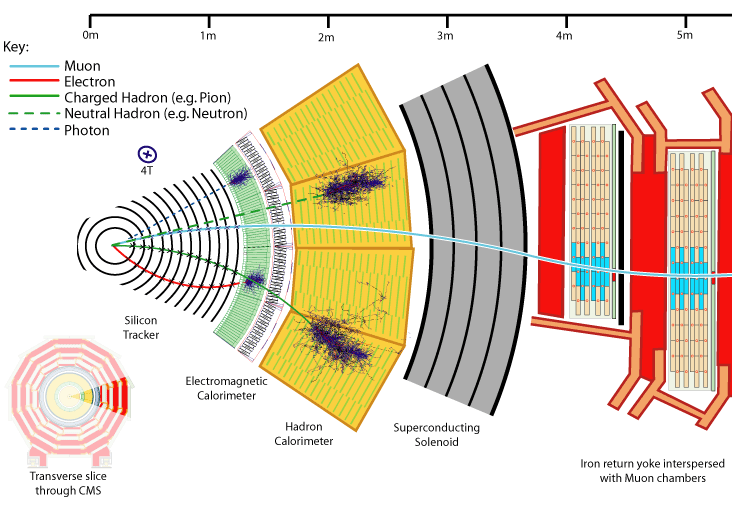
\includegraphics[width=0.6\columnwidth]{./cms12.png}
    \caption{Transverse view of the CMS detector showing the silicon tracker, electromagnetic calorimeter, hadron calorimeter, superconducting solenoid and muon chambers \cite{Chatrchyan:2008aa}.}
    \label{figure5}
  \end{figure}
  
  \begin{figure}[H]
    \centering
    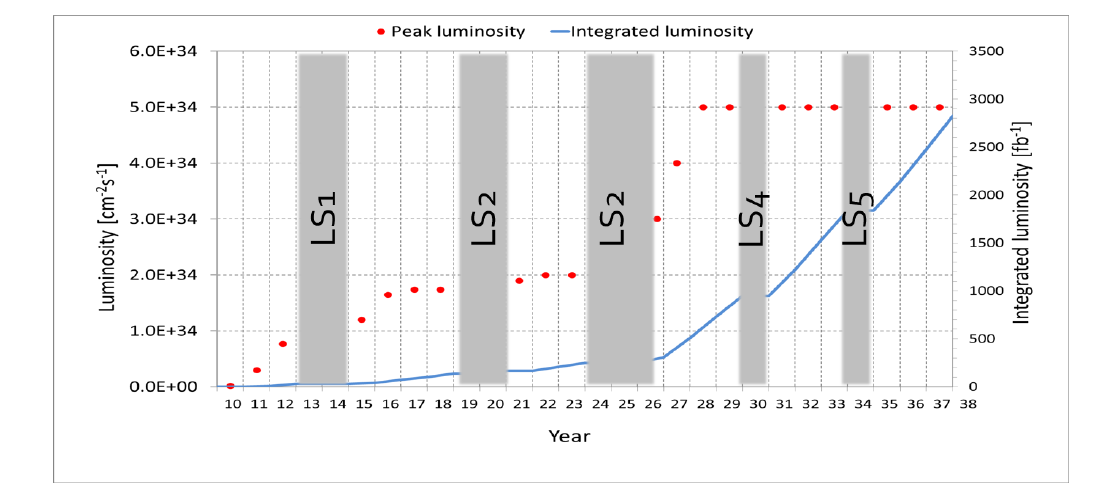
\includegraphics[width=0.9\columnwidth]{./lum6.png}
    \caption{Projected performance of the LHC until 2038, which shows the preliminary dates for prolonged stops (LS) of the LHC and luminosities. Points show instantaneous luminosity while the line shows luminosity accumulated \cite{collaborations2019report}.}
    \label{figure6}
  \end{figure}
  \clearpage


%\clearpage

LHC during the first run in 2011 and 2012 reached a peak instantaneous luminosity of 7.7 $\times$ $10^{33}$ $cm^{-2}s^{-1}$ which was more than 75$\%$ of its design luminosity and delivered an integrated luminosity of about 25 $fb^{-1}$ to each ATLAS and CMS.
 The LHC will deliver about 300 $fb^{-1}$ by 2024 \cite{collaborations2019report}.
The goal of subsequently run of LHC has been to obtain datasets at higher values of luminosities for precision measurements of the properties of Higgs boson, in order to test the Standard Model pattern of couplings to elementary particles.
In order to minimize the machine downtimes and maximize the productive use of the LHC for physics, the replacement of the inner triplet magnets (the one responsible to squeeze the beam at collision) and  of  all  hardware  changes  needed  to  enable  an  ambitious  luminosity  upgrade  will  take  place in parallel during one shutdown, at around 2023-25 (LS3), with some of the modification anticipated in 2019-2020 (LS2).
This new phase of the LHC life has been named as High Luminosity LHC (HL-LHC) and has the scope of attaining the astonishing threshold of 3000 $fb^{-1}$ by the year 2036 as shown in Figure~\ref{figure6}.
Figure~\ref{figureKappas} shows a summary of the current measurements of the Higgs coupling parameters with the LHC Run 1 dataset (2011,2012)  using ggF, VBF, VH, and ${t\bar{t}H}$ production modes \cite{Tanabashi:2018oca}.
Higgs boson production in association with single top quark has been studied to derive constraints on the magnitude and relative sign of Higgs boson couplings to top quarks and vector bosons.
Constaints on $\kappa_t$ can be derived using a likelihood ratio scan of $L(\kappa_t)/L(\hat{\kappa_t})$ where $\hat{\kappa_t}$ is the best fit value of $\kappa_t$ as shown in Figure~\ref{figureKt} \cite{Sirunyan:2018lzm}.
Multilepton final states like ee, $\mu\mu$ and $e\mu$ and final states with single lepton with a pair of bottom quarks were combined with Higgs decay to two photons to get the final result. The data slightly favor positive value of top quark yukawa coupling for SM Higgs boson and excludes ranges outside the intervals [-0.9,-0.5] and [1.0,2.1] times $y^{SM}_t$ at the 95 $\%$ confidence level.
\newpage
%\afterpage{
  \begin{figure}[H]
    \centering
    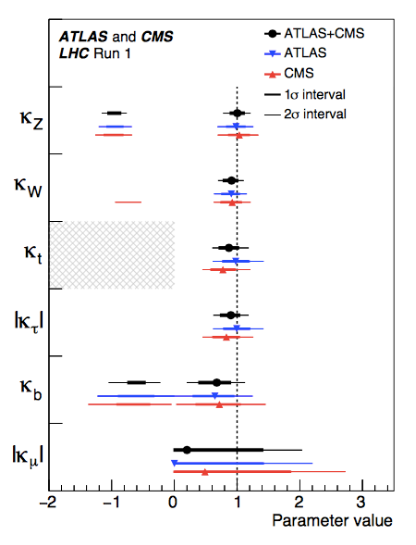
\includegraphics[scale=0.4]{./couplings.png}
    \caption{ATLAS-CMS combined measurements of coupling strength modifiers \cite{Tanabashi:2018oca}.}
    \label{figureKappas}
  \end{figure}
  
  \begin{figure}[H]
    \centering
    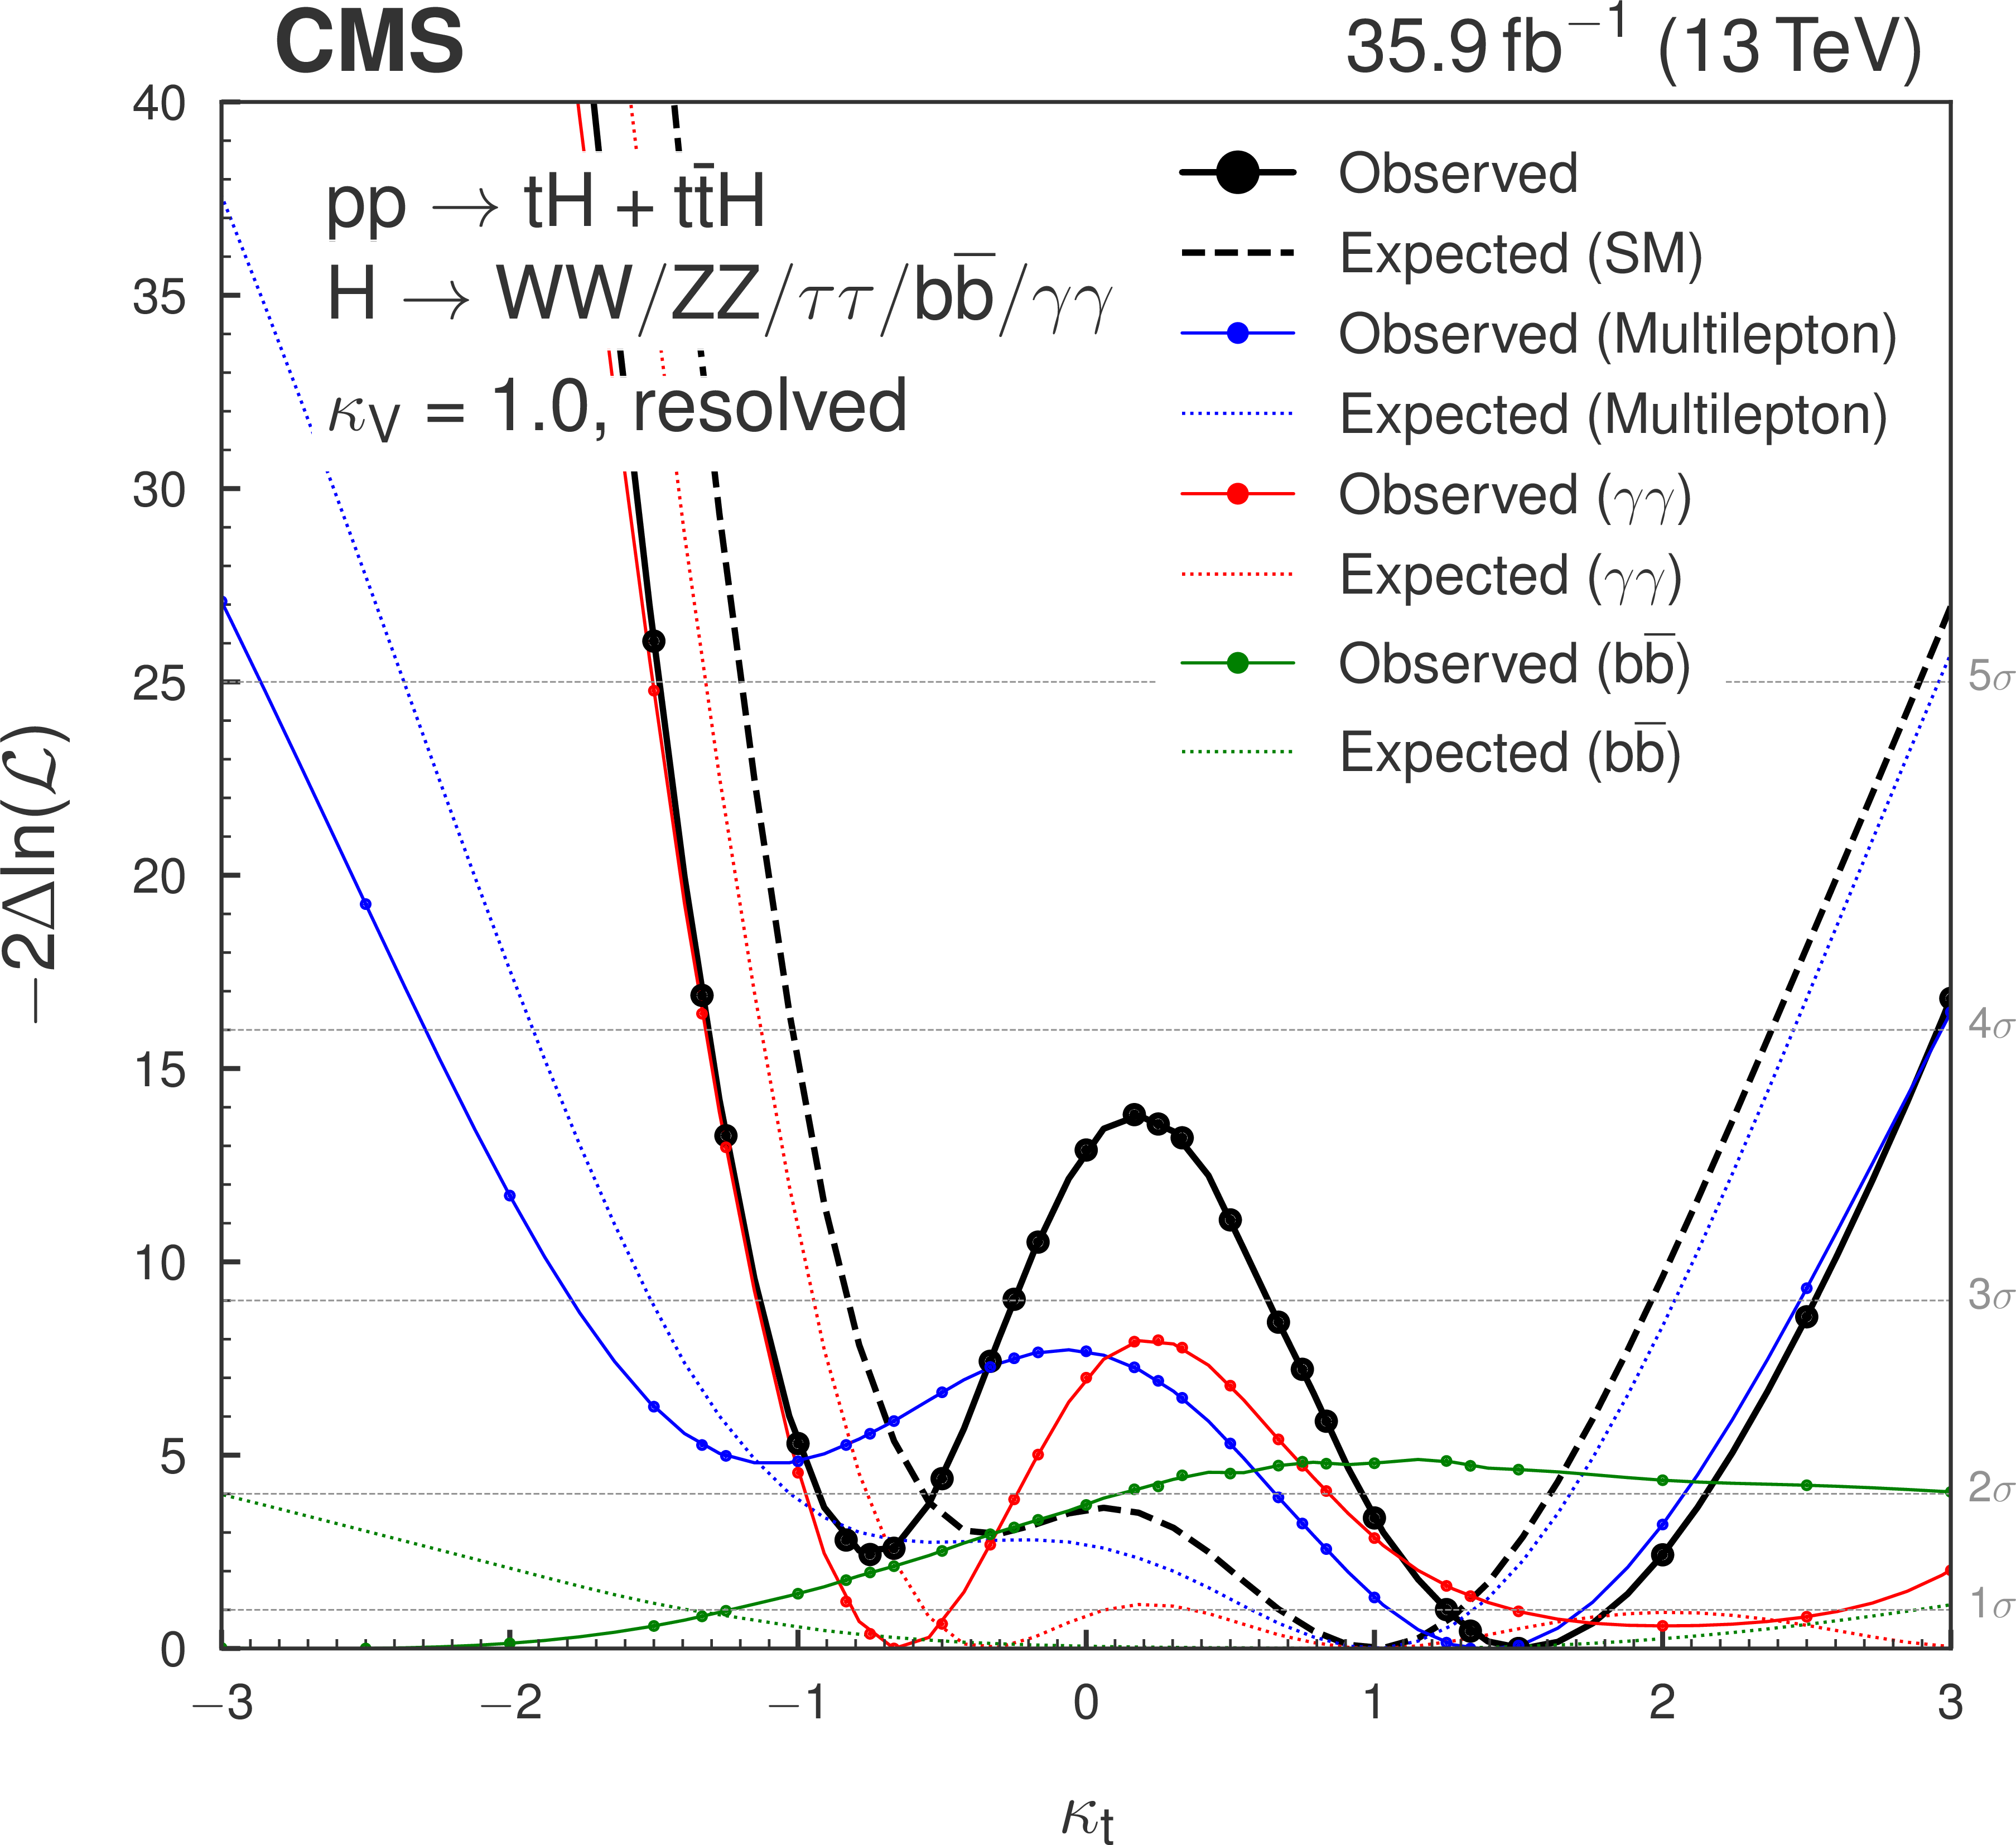
\includegraphics[width=0.4 \columnwidth]{./cms13.png}
    \caption{Scan of -2 $\Delta$ ln(L) versus $\kappa_t$ for the 2016 LHC data (black line) and the individual channels (blue, red, and green), compared to Asimov data sets corresponding to the SM expectations (dashed lines) \cite{sirunyan2019search}.}
    \label{figureKt}
  \end{figure}
  
\newpage
\section{PROPOSAL}

\onehalfspacing In this project, it is proposed to search for the production of Higgs boson associated with a single top quark in the CMS detector based at the Large Hadron Collider of the CERN laboratory.
It is proposed to study the sensitivity with the current data in the channel where the events are identified with two muons of the same sign, electron muon or with three leptons of electron or muon type.
Leptons of tau type are not considered due to complications in their identification in the detector.
%The impact of uncertainties will be studied and projections will be  made to the future phases of the LHC.
For these studies the data of the LHC Run 2 (2015-2018) will be used corresponding to an integrated luminosity of about 150 fb$^{-1}$, this is 4 times larger than the dataset used for current results.
It is also expected to estimate projections of the sensitivity to the High Luminosity phase of the LHC (HL-LHC) (2026-2036) which will accumulate up to 100 times the data used for current measurements. 


\section{GENERAL OBJECTIVE}

%- motivation, tH production crossection, sign of $k_t$, search for BSM, ..

\onehalfspacing There is currently a great enigma in physics since we know that ordinary matter comprises only $5\%$ of the universe, another $27\%$ includes Dark matter and the rest $68\%$ is Dark energy.
Understanding the production of the Higgs boson, as well as its decays are an important part of the physics program of CERN laboratory experiments to verify the Standard Model and look for new particles. Through this project we will investigate the production of the Higgs boson in association with a single top quark (tH) in proton-proton collisions with the CMS experiment at the LHC. The tH  production process has not been observed so far.
The measurement of this process complements other measurements of the yukawa coupling parameter $y_t$ of the top quark and Higgs boson and is a part of the physics program of CMS and ATLAS international collaborations. Through these measurements we seek to complete the measurements of the Standard Model parameters to high precision and also to find evidence of deviations in yukawa couplings which point to new particles which may explain current enigmas like the origin of Dark Matter.


\section{HYPOTHESIS}
%%  - what we expect to find

\onehalfspacing Studies about the tH Higgs boson production channel have already started within the CMS and ATLAS collaboration and publications are based on data from the 2011-2012 run and some data from the second run of 2015-2016.
In these results, there was no evidence of signal and upper limits were set on the production cross-section.
The current results combine three types of searches: H$\rightarrow WW/ZZ/\tau\tau \rightarrow$leptons, H$\rightarrow\gamma\gamma$, and H$\rightarrow b\bar{b}$.
%The most sensitive channel is  with leptons, however this channel is a combination of two sub-channels: two-lepton and three-lepton.
The currently published result uses 36 fb$^{-1}$ of collision data and obtains an upper limit of 2.04 pb while only 0.077 pb are expected in the SM \cite{sirunyan2019search}, the limit is 26 times larger than the expected value.
In BSM models, for example with $\kappa_t = -1$,  the expected cross-section increases up to 0.834 pb due to quantum interference effects; in this case also the observed upper limit changes to 0.86 pb at 95$\%$ confidence level, the current data almost rules out this model.  

With this project we propose to incorporate the full Run 2 dataset corresponding to 150 fb$^{-1}$.
A factor of 4 increase in number of collision events will improve the limits by a factor of approximately 2 due to the nature of statistical uncertainties.
This mean that the limit for the SM case will improve to about 13 times the expected cross-section, while for the modified model ($\kappa_t = -1$) we expect to be excluded.

Additionally, in subsequent phases of the LHC (2021-2023 and 2026-2038) the amount of data will increase by a factor of up to 100, which implies the upper limit for the SM case will reduce to about 2.6 times the expected cross-section. This implies that even for the HL-LHC it will be difficult to observe the tH production, but at the same time more and more phase space of BSM models will be excluded.  

In this search the reconstruction methods do not allow to separate $t$H from $t\bar{t}H$ production because the cross-section of $t\bar{t}H$ is much larger than that of tH and some events pass the selections designed for tH.
The fraction of tH events over tH + $t\bar{t}H$ is currently only 5$\%$ with the analysis techniques used.
We expect to improve the analysis techniques using multi-variate techniques, for example boosted decision trees or other algorithms, to improve the identification of signal events over the rest of the backgrounds.
This will provide additional improvements in the limits and a possible observation of the SM signal as well as stringent exclusions for BSM models.

%\newpage
\section{SPECIFIC OBJECTIVES}

\onehalfspacing The measurement of the tH production mechanism is a collaborative effort in the LHC experiment due to the various channels that need to be combined.
This project focuses on the channels with leptons in the final state: two-lepton ($\ell\ell$) or three-lepton ($\ell\ell\ell$).
The $\ell\ell$ sub-channel uses events with same sign dimuon ($\mu^\pm\mu^\pm$) or electron-muon ($e^\pm\mu^\pm$).
The $\ell\ell\ell$ sub-channel uses events in the topologies: $\mu\mu\mu$, $\mu\mu e$, $\mu e e$ and $e e e$, where no charge requirements are made.
The leptons are generated from the decays of the $W$ and $Z$ bosons or $\tau$ leptons from decays of the Higgs or top quarks.
Furthermore, light-quark and b-quark jets are generated from the initial state collision and from the decay of the top quark, these must be used in the signal identification.

In order to complete a journal publication of a  measurement of tH production using one of these channels, several aspects  must be worked on:
\begin{itemize}
\item Simulation of the signal events using Monte Carlo generators which implement the theoretical model.
\item Implementation of event reconstruction and selection algorithms which select high quality signal events and reduce the background events to a minimum.
\item Studies of lepton and jet identification algorithms which improve the background rejection.
\item Due to the small signal over background ratio, a multi-variate algorithm is employed which combines different event variables and exploits the correlations to construct a final discriminant. This algorithm must be trained using simulated signal and background events.
\item A model for the observed data must be constructed from the known background processes. These processes are normally simulated individually and then summed together with the signal to construct the final statistical model.
\item An algorithm is developed that adjusts the model to the observed data distribution and incorporates several systematic uncertainties due to differences between simulation and real data.
\item The signal strength observed from the statistical analysis must be interpreted as evidence of a signal or in the absence as a limit. Further analysis is required to place constraints on paramater space of BSM models.
\end{itemize}

In addition to the above objectives, members of the CMS collaboration are expected to participate in the detector operation and upgrade activities (or service work).
During shut-down periods, these activities include testing and installation of new detectors.
During regular data-taking periods, activities include monitoring the data acquisition systems and data quality through comparisons of new data and old data.
In addition to the data analysis plans described before, another objective is to contribute in one of the developments of the CMS detector to  prepare for the HL-LHC phase.
%

Finally, the results of this project will be presented at national or international conferences and a publication in a scientific journal will be accomplished.


\section{METHODOLOGY}
%- methods used in the search: which dataset,  lepton reconstruction, selections, jets, BDT, backgrounds, statistical analysis


%\afterpage{
%\begin{figure}[H]
%	\centering
%	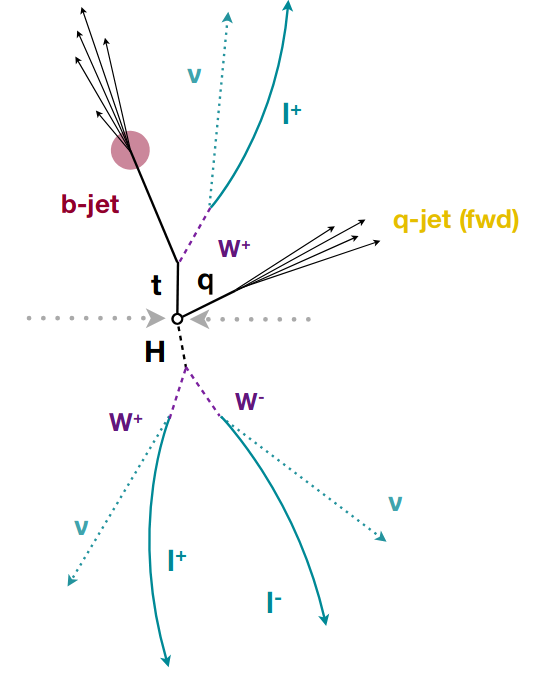
\includegraphics[width=0.5\columnwidth]{./topology.png}
%	\caption{Topology of a tH signal event in a proton-proton collision. The decay products from the top quark include a b-jet and a W boson decaying to a lepton and neutrino. In this diagram the Higgs decays to a pair of W bosons, one decays to a lepton and neutrino while the other one can decay leptonically or hadronically. In addition there is a forward jet from initial collision of the quarks.}
%	\label{figureTopology}
%\end{figure}
%\clearpage



\onehalfspacing The methods for a measurement of the coupling of the Higgs boson and the top quark in proton collisions are extensive and require several stages.

Accelerating the protons to extremely high energies and causing them to collide at high rates in order to produce rare but interesting events is the work of a separate accelerator group.
However, the members of the CMS collaboration must monitor the quality and rate of proton collisions at the interaction point at the center of the detector in order to collect a high quality dataset which can be stored for many years to do analysis.
Calibration and maintenance of all parts of the detector is necessary in order to achieve close to $100\%$ particle detection efficiency and noise levels to a minimum. This work is achieved by participating in the detector operation groups and performing data acquisition shifts during run time.  
Presence at CERN or at a remote control center like Fermilab is required in order to perform these activities. 


The reconstruction and selection of signal events is studied using the \textsc{MadGraph}~\cite{alwall2014automated} Monte Carlo generator which implements the theoretical model and predict the amount and distribution of events for a given LHC dataset.


\begin{figure}[H]
	\centering
	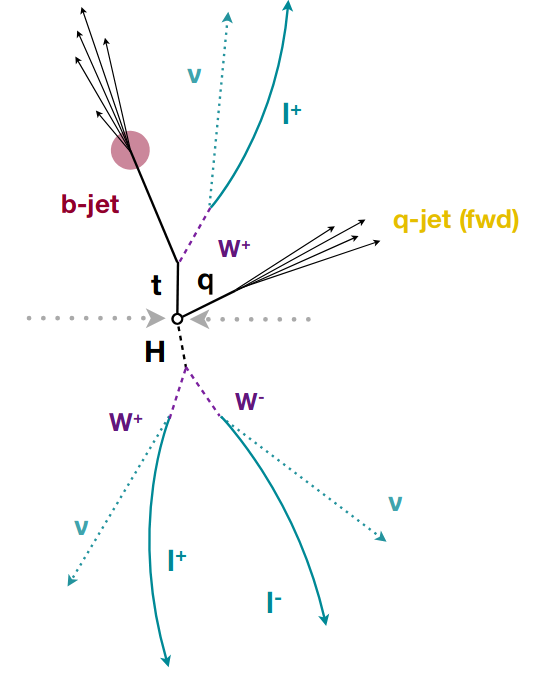
\includegraphics[width=0.5\columnwidth]{./topology.png}
	\caption{Topology of a tH signal event in a proton-proton collision. The decay products from the top quark include a b-jet and a $W^{\pm}$ boson decaying to a lepton and neutrino. In this diagram the Higgs decays to a pair of $W^{\pm}$ bosons, one decays to a lepton and neutrino while the other one can decay leptonically or hadronically. In addition there is a forward jet from initial collision of the quarks.}
	\label{figureTopology}
\end{figure}
Figure~\ref{figureTopology} shows the main features of the topology of a tH event, including the subsequent decay products of the top quark and Higgs boson, these are the particles which are generated at the interaction point before entering the detector components.
A separate simulation of the detector is employed using \textsc{Geant}~\cite{agostinelli2003geant4} which simulates the trajectory of the stable particles, response and efficiency of each sensor in the CMS detector.
The information obtained from this chain is saved as raw data similar to the one obtained from the real experiment and is later reconstructed in the same way.

The event reconstruction is designed to capture the distinguishing features of the signal topology.
In the channels which are the focus of this project, we require that there exist at least two leptons of electron or muon type, however also jets need to be identified as shown in the Figure 9.
The event reconstruction begins with the identification of the different types of particles: photon, electrons, muons, taus, and jets.
Particle lists are formed for each kind using a general purpose event reconstruction software called \textsc{CMSSW}~\cite{Bayatian:922757} which is maintained by the collaboration and which includes basic calibration of the various particle energy and momenta.

The Tracker subdetector of CMS shown in Figure~\ref{figure5} is composed of silicon sensors which detect minimum ionizing charged particles coming from the interaction region. The Tracker consists of an inner Pixel detector with layers of pixel sensors and an outer Strip detector. The Pixel system consists of 66 Million pixels while the Strip system comprises of 9.6 Million strip sensors. The Tracker provides a precision measurement of the track curvature (momentum) and position at the interaction region.

Electrons are reconstructed from clusters of energy in the Electromagnetic calorimeter (ECAL). The ECAL is made of rectangular transparent crystals which cause a shower of secondary photons and electrons. The energy deposited in the crystal is read out and determines the energy of the primary electron. The cluster must match to a track in the Tracker subdetector. Photons are similar to electrons, but a track must not be matched in this case.

Muons are identified by tracks which exit the inner subdetectors and cross the solenoid into the Muon chambers. Drift Tubes (DT's) in the barrel region or Cathode Strip Chambers (CSC's) in the forward region use ionizing gas to detect the passage of muon tracks.  The track in the Muon chambers is matched to the track in the Tracker to provide a measurement of the muon momentum.

Jets are reconstructed from energetic clusters found in both the ECAL and the Hadronic calorimeter (HCAL).
Pions, kaons, and other hadrons create showers of secondary particles in the dense metal plates of the HCAL, the ionization energy of secondary particles is read out with scintillating plastics interleaved with the metal plates.  
Jets originate at the interaction region from collisions of quarks and gluons which create showers of mesons and baryons (mainly pions).
Jets which originate from b quarks are important in this study because they identify the decay of a top quark, b-jets are identified with a multivariate algorithm which searches for secondary vertices in the Tracker and electrons or muons (from decays of B-mesons) within the cone of the jet.

A new data structure with the above particle reconstruction defines new  datasets (\textsc{CMSSW}) stored in computing centers around the world which are available to students and scientists at all research institutions.
These  datasets are processed using computing clusters which use high-performance computing systems, normally using HTCondor~\cite{HTCondor} to link the processing nodes, which allows hundreds of jobs to run at the same time by individual users and save the output in \textsc{Root} format \cite{brun2003root}.
In this processing, the particle lists are used to require certain event selections and filter out uninteresting events.

In the search for tH events using the dimuon channel the following event selections are applied:
\begin{itemize}
\item exactly two muons with the same sign,
\item leading muon with at least 25 GeV,
\item sub-leading muon with at least 15 GeV,
\item at least one b-tagged jet,
  \item and at least one non-b-tagged jet.
\end{itemize}


\textsc{Root} is a \textsc{c++} based software that allows visualization of event distributions and variable correlations.
Further optimization of the event selections is performed by considering the different processes which contribute to the background.
In this search several SM processes contribute to the background due to their decays to leptons: $pp\rightarrow ZZ, WZ, WW, ZZZZ, t\bar{t}W, t\bar{t}Z, t\bar{t}H, tWZ, tZq,$ and $t\bar{t}t\bar{t}$.
These backgrounds must be determined from MC simulation and normalized to their predicted SM cross sections. 

Due to the small signal over noise ratio in this search, a multivariate algorithm is trained to help separate signal events from background events.
A typical algorithm used is the Boosted Decision Tree~\cite{hoecker2007tmva}, which takes as input several event variables related to the signal topology.
In the previous search for tH these variables included:
\begin{itemize}
\item rapidity of the most forward jet,
\item momentum of the sub-leading lepton,
\item number of central jets,
\item number of forward jets,
\item and other angular variables between the jets and leptons.
\end{itemize}
The multivariate algorithm takes into account the correlations between the variables and combines the information into a single discriminant.

Due to the maximum separation of the signal and background in the multivariate discriminant, this distribution is used for the statisical analysis of the events.
A fit is applied using the \textsc{RooFit} software package~\cite{verkerke2008roofit} which constructs a model for the data consisting of the sum of the backgrounds and the signal simulations. A likelihood function is constructed from a Poisson function using the expected and measured number of events.
Systematic uncertainties are incorporated as nuisance parameters using gaussian probability functions, these account for uncertaintes in the normalization and shapes of the background.
The signal strength extracted from this fit determines if there is any evidence for a signal.
In the absence of a signal an upper limit is placed on the signal strength using the likelihood function and subsequently translated into a limit in the tH production cross section and the Higgs coupling parameters. 


\section{EXPECTED RESULTS}
%- a limit, also predictions for future runs

\onehalfspacing The results from this project include the following items:
\begin{itemize}
\item The student will become part of an international collaboration.
\item A leading contribution in one of the search channels for the tH process using the data from the Run II of the LHC, resulting in a publication in a scientific journal.
\item Participation in the CMS detector Phase II upgrade through development and possible installation of particle detectors possibly resulting in a technical report.
\item A presentation of a poster or a talk in one of the national conferences of the Division of Paticles and Fields of the Mexican Society of Physics or a presentation of a poster or a talk in an international physics conference.
\item An academic stay at a scientific center like CERN or Fermilab.
\item A high quality thesis.
\end{itemize}



\section{CALENDAR OF ACTIVITIES}
\onehalfspacing
\begin{itemize}
\item {\bf Semester 1 (2019-2)}:
  \SubItem{ Readings on Standard Model theory}
  \SubItem{ Basic Linux computing skills (\textsc{Bash, Emacs, Root})}
  \SubItem{ Initial planning of the analysis strategy}
\item {\bf Semester 2 (2020-1)}:
  \SubItem{ Course I on particle physics and/or particle detection}
  \SubItem{ Basic Linux computing skills (\textsc{Bash, Emacs, Root})}
  \SubItem{ Readings on SM and tH literature}
  \SubItem{ Computing accounts at CERN and Fermilab}
  \SubItem{ Studies of the tH event selections}
  \SubItem{ CMS service work for authorship}
  \SubItem{ Possible summer stay at CERN or Fermilab}
\item {\bf Semester 3 (2020-2)}:
  \SubItem{ Course II on particle physics and/or particle detection.}
  \SubItem{ Studies of the tH event selections}
  \SubItem{ Development of a Multivariate algorithm for the event selections}
  \SubItem{ Studies of the background processes}
  \SubItem{ CMS service work for authorship}
\item {\bf Semester 4 (2021-1)}:
  \SubItem{ CMS service work for authorship}
  \SubItem{ Studies of the tH event selections}
  \SubItem{ Development of a Multivariate algorithm for the event selections}
  \SubItem{ Studies of the tH background processes}
  \SubItem{ Development of the statistical model and signal extraction}
  \SubItem{ Possible summer stay at CERN or Fermilab}
\item {\bf Semester 5 (2021-2)}:
  \SubItem{ Studies of the tH event selections}
  \SubItem{ Development of a Multivariate algorithm for the event selections}
  \SubItem{ Studies of the tH background processes}
  \SubItem{ Development of the statistical model and signal extraction}
  \SubItem{ Presentation of poster or talk at national or international conference}
\item {\bf Semester 6 (2022-1)}:
  \SubItem{ Development of software for the statistical analysis and interpretation of the results}
  \SubItem{ Review process of the results within the CMS collaboration}
  \SubItem{ Presentation of poster or talk at national or international conference}
  \SubItem{ Writing of the paper publication}
  \SubItem{ Writing of the thesis}
\end{itemize}





\cleardoublepage
\onehalfspacing
\bibliographystyle{unsrt}
\bibliography{paper}

\end{document}

